
%% bare_jrnl.tex
%% V1.4b
%% 2015/08/26
%% by Michael Shell
%% see http://www.michaelshell.org/
%% for current contact information.
%%
%% This is a skeleton file demonstrating the use of IEEEtran.cls
%% (requires IEEEtran.cls version 1.8b or later) with an IEEE
%% journal paper.
%%
%% Support sites:
%% http://www.michaelshell.org/tex/ieeetran/
%% http://www.ctan.org/pkg/ieeetran
%% and
%% http://www.ieee.org/

%%*************************************************************************
%% Legal Notice:
%% This code is offered as-is without any warranty either expressed or
%% implied; without even the implied warranty of MERCHANTABILITY or
%% FITNESS FOR A PARTICULAR PURPOSE! 
%% User assumes all risk.
%% In no event shall the IEEE or any contributor to this code be liable for
%% any damages or losses, including, but not limited to, incidental,
%% consequential, or any other damages, resulting from the use or misuse
%% of any information contained here.
%%
%% All comments are the opinions of their respective authors and are not
%% necessarily endorsed by the IEEE.
%%
%% This work is distributed under the LaTeX Project Public License (LPPL)
%% ( http://www.latex-project.org/ ) version 1.3, and may be freely used,
%% distributed and modified. A copy of the LPPL, version 1.3, is included
%% in the base LaTeX documentation of all distributions of LaTeX released
%% 2003/12/01 or later.
%% Retain all contribution notices and credits.
%% ** Modified files should be clearly indicated as such, including  **
%% ** renaming them and changing author support contact information. **
%%*************************************************************************


% *** Authors should verify (and, if needed, correct) their LaTeX system  ***
% *** with the testflow diagnostic prior to trusting their LaTeX platform ***
% *** with production work. The IEEE's font choices and paper sizes can   ***
% *** trigger bugs that do not appear when using other class files.       ***                          ***
% The testflow support page is at:
% http://www.michaelshell.org/tex/testflow/



\documentclass[journal]{IEEEtran}
%
% If IEEEtran.cls has not been installed into the LaTeX system files,
% manually specify the path to it like:
% \documentclass[journal]{../sty/IEEEtran}

\usepackage{graphicx}
\usepackage{subcaption}
\usepackage{pgfplotstable}
\usepackage{pgfplots}
\usepackage{amsmath}
\usepackage{amssymb}
\usepackage{amstext}
\usepackage{amsfonts}
\usepackage{mathrsfs}
\usepackage[section]{placeins}
\usepackage{multicol}


\definecolor{Square_Large}{RGB}{255,0,0}
\definecolor{Square_Small}{RGB}{155,0,0}
\definecolor{Chess_Large}{RGB}{0,0,255}
\definecolor{Chess_Small}{RGB}{0,0,155}


\definecolor{ICC}{RGB}{0,255,255}
\definecolor{PBD}{RGB}{255,0,155}
\definecolor{DICE}{RGB}{0,255,0}
\definecolor{JAC}{RGB}{0,155,0}
\definecolor{FMS}{RGB}{0,55,0}

\definecolor{HD}{RGB}{155,0,255}
\definecolor{AVD}{RGB}{155,155,255}
\definecolor{MHD}{RGB}{55,0,255}

\definecolor{KAP}{RGB}{0,0,0}
\definecolor{AUC}{RGB}{155,155,155}


% Some very useful LaTeX packages include:
% (uncomment the ones you want to load)


% *** MISC UTILITY PACKAGES ***
%
%\usepackage{ifpdf}
% Heiko Oberdiek's ifpdf.sty is very useful if you need conditional
% compilation based on whether the output is pdf or dvi.
% usage:
% \ifpdf
%   % pdf code
% \else
%   % dvi code
% \fi
% The latest version of ifpdf.sty can be obtained from:
% http://www.ctan.org/pkg/ifpdf
% Also, note that IEEEtran.cls V1.7 and later provides a builtin
% \ifCLASSINFOpdf conditional that works the same way.
% When switching from latex to pdflatex and vice-versa, the compiler may
% have to be run twice to clear warning/error messages.






% *** CITATION PACKAGES ***
%
%\usepackage{cite}
% cite.sty was written by Donald Arseneau
% V1.6 and later of IEEEtran pre-defines the format of the cite.sty package
% \cite{} output to follow that of the IEEE. Loading the cite package will
% result in citation numbers being automatically sorted and properly
% "compressed/ranged". e.g., [1], [9], [2], [7], [5], [6] without using
% cite.sty will become [1], [2], [5]--[7], [9] using cite.sty. cite.sty's
% \cite will automatically add leading space, if needed. Use cite.sty's
% noadjust option (cite.sty V3.8 and later) if you want to turn this off
% such as if a citation ever needs to be enclosed in parenthesis.
% cite.sty is already installed on most LaTeX systems. Be sure and use
% version 5.0 (2009-03-20) and later if using hyperref.sty.
% The latest version can be obtained at:
% http://www.ctan.org/pkg/cite
% The documentation is contained in the cite.sty file itself.






% *** GRAPHICS RELATED PACKAGES ***
%
\ifCLASSINFOpdf
  % \usepackage[pdftex]{graphicx}
  % declare the path(s) where your graphic files are
  % \graphicspath{{../pdf/}{../jpeg/}}
  % and their extensions so you won't have to specify these with
  % every instance of \includegraphics
  % \DeclareGraphicsExtensions{.pdf,.jpeg,.png}
\else
  % or other class option (dvipsone, dvipdf, if not using dvips). graphicx
  % will default to the driver specified in the system graphics.cfg if no
  % driver is specified.
  % \usepackage[dvips]{graphicx}
  % declare the path(s) where your graphic files are
  % \graphicspath{{../eps/}}
  % and their extensions so you won't have to specify these with
  % every instance of \includegraphics
  % \DeclareGraphicsExtensions{.eps}
\fi
% graphicx was written by David Carlisle and Sebastian Rahtz. It is
% required if you want graphics, photos, etc. graphicx.sty is already
% installed on most LaTeX systems. The latest version and documentation
% can be obtained at: 
% http://www.ctan.org/pkg/graphicx
% Another good source of documentation is "Using Imported Graphics in
% LaTeX2e" by Keith Reckdahl which can be found at:
% http://www.ctan.org/pkg/epslatex
%
% latex, and pdflatex in dvi mode, support graphics in encapsulated
% postscript (.eps) format. pdflatex in pdf mode supports graphics
% in .pdf, .jpeg, .png and .mps (metapost) formats. Users should ensure
% that all non-photo figures use a vector format (.eps, .pdf, .mps) and
% not a bitmapped formats (.jpeg, .png). The IEEE frowns on bitmapped formats
% which can result in "jaggedy"/blurry rendering of lines and letters as
% well as large increases in file sizes.
%
% You can find documentation about the pdfTeX application at:
% http://www.tug.org/applications/pdftex





% *** MATH PACKAGES ***
%
%\usepackage{amsmath}
% A popular package from the American Mathematical Society that provides
% many useful and powerful commands for dealing with mathematics.
%
% Note that the amsmath package sets \interdisplaylinepenalty to 10000
% thus preventing page breaks from occurring within multiline equations. Use:
%\interdisplaylinepenalty=2500
% after loading amsmath to restore such page breaks as IEEEtran.cls normally
% does. amsmath.sty is already installed on most LaTeX systems. The latest
% version and documentation can be obtained at:
% http://www.ctan.org/pkg/amsmath





% *** SPECIALIZED LIST PACKAGES ***
%
%\usepackage{algorithmic}
% algorithmic.sty was written by Peter Williams and Rogerio Brito.
% This package provides an algorithmic environment fo describing algorithms.
% You can use the algorithmic environment in-text or within a figure
% environment to provide for a floating algorithm. Do NOT use the algorithm
% floating environment provided by algorithm.sty (by the same authors) or
% algorithm2e.sty (by Christophe Fiorio) as the IEEE does not use dedicated
% algorithm float types and packages that provide these will not provide
% correct IEEE style captions. The latest version and documentation of
% algorithmic.sty can be obtained at:
% http://www.ctan.org/pkg/algorithms
% Also of interest may be the (relatively newer and more customizable)
% algorithmicx.sty package by Szasz Janos:
% http://www.ctan.org/pkg/algorithmicx




% *** ALIGNMENT PACKAGES ***
%
%\usepackage{array}
% Frank Mittelbach's and David Carlisle's array.sty patches and improves
% the standard LaTeX2e array and tabular environments to provide better
% appearance and additional user controls. As the default LaTeX2e table
% generation code is lacking to the point of almost being broken with
% respect to the quality of the end results, all users are strongly
% advised to use an enhanced (at the very least that provided by array.sty)
% set of table tools. array.sty is already installed on most systems. The
% latest version and documentation can be obtained at:
% http://www.ctan.org/pkg/array


% IEEEtran contains the IEEEeqnarray family of commands that can be used to
% generate multiline equations as well as matrices, tables, etc., of high
% quality.




% *** SUBFIGURE PACKAGES ***
%\ifCLASSOPTIONcompsoc
%  \usepackage[caption=false,font=normalsize,labelfont=sf,textfont=sf]{subfig}
%\else
%  \usepackage[caption=false,font=footnotesize]{subfig}
%\fi
% subfig.sty, written by Steven Douglas Cochran, is the modern replacement
% for subfigure.sty, the latter of which is no longer maintained and is
% incompatible with some LaTeX packages including fixltx2e. However,
% subfig.sty requires and automatically loads Axel Sommerfeldt's caption.sty
% which will override IEEEtran.cls' handling of captions and this will result
% in non-IEEE style figure/table captions. To prevent this problem, be sure
% and invoke subfig.sty's "caption=false" package option (available since
% subfig.sty version 1.3, 2005/06/28) as this is will preserve IEEEtran.cls
% handling of captions.
% Note that the Computer Society format requires a larger sans serif font
% than the serif footnote size font used in traditional IEEE formatting
% and thus the need to invoke different subfig.sty package options depending
% on whether compsoc mode has been enabled.
%
% The latest version and documentation of subfig.sty can be obtained at:
% http://www.ctan.org/pkg/subfig




% *** FLOAT PACKAGES ***
%
%\usepackage{fixltx2e}
% fixltx2e, the successor to the earlier fix2col.sty, was written by
% Frank Mittelbach and David Carlisle. This package corrects a few problems
% in the LaTeX2e kernel, the most notable of which is that in current
% LaTeX2e releases, the ordering of single and double column floats is not
% guaranteed to be preserved. Thus, an unpatched LaTeX2e can allow a
% single column figure to be placed prior to an earlier double column
% figure.
% Be aware that LaTeX2e kernels dated 2015 and later have fixltx2e.sty's
% corrections already built into the system in which case a warning will
% be issued if an attempt is made to load fixltx2e.sty as it is no longer
% needed.
% The latest version and documentation can be found at:
% http://www.ctan.org/pkg/fixltx2e


%\usepackage{stfloats}
% stfloats.sty was written by Sigitas Tolusis. This package gives LaTeX2e
% the ability to do double column floats at the bottom of the page as well
% as the top. (e.g., "\begin{figure*}[!b]" is not normally possible in
% LaTeX2e). It also provides a command:
%\fnbelowfloat
% to enable the placement of footnotes below bottom floats (the standard
% LaTeX2e kernel puts them above bottom floats). This is an invasive package
% which rewrites many portions of the LaTeX2e float routines. It may not work
% with other packages that modify the LaTeX2e float routines. The latest
% version and documentation can be obtained at:
% http://www.ctan.org/pkg/stfloats
% Do not use the stfloats baselinefloat ability as the IEEE does not allow
% \baselineskip to stretch. Authors submitting work to the IEEE should note
% that the IEEE rarely uses double column equations and that authors should try
% to avoid such use. Do not be tempted to use the cuted.sty or midfloat.sty
% packages (also by Sigitas Tolusis) as the IEEE does not format its papers in
% such ways.
% Do not attempt to use stfloats with fixltx2e as they are incompatible.
% Instead, use Morten Hogholm'a dblfloatfix which combines the features
% of both fixltx2e and stfloats:
%
% \usepackage{dblfloatfix}
% The latest version can be found at:
% http://www.ctan.org/pkg/dblfloatfix




%\ifCLASSOPTIONcaptionsoff
%  \usepackage[nomarkers]{endfloat}
% \let\MYoriglatexcaption\caption
% \renewcommand{\caption}[2][\relax]{\MYoriglatexcaption[#2]{#2}}
%\fi
% endfloat.sty was written by James Darrell McCauley, Jeff Goldberg and 
% Axel Sommerfeldt. This package may be useful when used in conjunction with 
% IEEEtran.cls'  captionsoff option. Some IEEE journals/societies require that
% submissions have lists of figures/tables at the end of the paper and that
% figures/tables without any captions are placed on a page by themselves at
% the end of the document. If needed, the draftcls IEEEtran class option or
% \CLASSINPUTbaselinestretch interface can be used to increase the line
% spacing as well. Be sure and use the nomarkers option of endfloat to
% prevent endfloat from "marking" where the figures would have been placed
% in the text. The two hack lines of code above are a slight modification of
% that suggested by in the endfloat docs (section 8.4.1) to ensure that
% the full captions always appear in the list of figures/tables - even if
% the user used the short optional argument of \caption[]{}.
% IEEE papers do not typically make use of \caption[]'s optional argument,
% so this should not be an issue. A similar trick can be used to disable
% captions of packages such as subfig.sty that lack options to turn off
% the subcaptions:
% For subfig.sty:
% \let\MYorigsubfloat\subfloat
% \renewcommand{\subfloat}[2][\relax]{\MYorigsubfloat[]{#2}}
% However, the above trick will not work if both optional arguments of
% the \subfloat command are used. Furthermore, there needs to be a
% description of each subfigure *somewhere* and endfloat does not add
% subfigure captions to its list of figures. Thus, the best approach is to
% avoid the use of subfigure captions (many IEEE journals avoid them anyway)
% and instead reference/explain all the subfigures within the main caption.
% The latest version of endfloat.sty and its documentation can obtained at:
% http://www.ctan.org/pkg/endfloat
%
% The IEEEtran \ifCLASSOPTIONcaptionsoff conditional can also be used
% later in the document, say, to conditionally put the References on a 
% page by themselves.




% *** PDF, URL AND HYPERLINK PACKAGES ***
%
%\usepackage{url}
% url.sty was written by Donald Arseneau. It provides better support for
% handling and breaking URLs. url.sty is already installed on most LaTeX
% systems. The latest version and documentation can be obtained at:
% http://www.ctan.org/pkg/url
% Basically, \url{my_url_here}.




% *** Do not adjust lengths that control margins, column widths, etc. ***
% *** Do not use packages that alter fonts (such as pslatex).         ***
% There should be no need to do such things with IEEEtran.cls V1.6 and later.
% (Unless specifically asked to do so by the journal or conference you plan
% to submit to, of course. )


% correct bad hyphenation here
\hyphenation{op-tical net-works semi-conduc-tor}


\begin{document}
%
% paper title
% Titles are generally capitalized except for words such as a, an, and, as,
% at, but, by, for, in, nor, of, on, or, the, to and up, which are usually
% not capitalized unless they are the first or last word of the title.
% Linebreaks \\ can be used within to get better formatting as desired.
% Do not put math or special symbols in the title.
\title{Evaluation of Evaluation Metrics}
%
%
% author names and IEEE memberships
% note positions of commas and nonbreaking spaces ( ~ ) LaTeX will not break
% a structure at a ~ so this keeps an author's name from being broken across
% two lines.
% use \thanks{} to gain access to the first footnote area
% a separate \thanks must be used for each paragraph as LaTeX2e's \thanks
% was not built to handle multiple paragraphs
%

\author{Grimm Lorenz
        and~Rohrbach Simon% <-this % stops a space
\thanks{}% <-this % stops a space
\thanks{}% <-this % stops a space
\thanks{}}

% note the % following the last \IEEEmembership and also \thanks - 
% these prevent an unwanted space from occurring between the last author name
% and the end of the author line. i.e., if you had this:
% 
% \author{....lastname \thanks{...} \thanks{...} }
%                     ^------------^------------^----Do not want these spaces!
%
% a space would be appended to the last name and could cause every name on that
% line to be shifted left slightly. This is one of those "LaTeX things". For
% instance, "\textbf{A} \textbf{B}" will typeset as "A B" not "AB". To get
% "AB" then you have to do: "\textbf{A}\textbf{B}"
% \thanks is no different in this regard, so shield the last } of each \thanks
% that ends a line with a % and do not let a space in before the next \thanks.
% Spaces after \IEEEmembership other than the last one are OK (and needed) as
% you are supposed to have spaces between the names. For what it is worth,
% this is a minor point as most people would not even notice if the said evil
% space somehow managed to creep in.



% The paper headers
\markboth{Evaluation of Evaluation Metrics, January~2018}%
{Shell \MakeLowercase{\textit{et al.}}: Bare Demo of IEEEtran.cls for IEEE Journals}
% The only time the second header will appear is for the odd numbered pages
% after the title page when using the twoside option.
% 
% *** Note that you probably will NOT want to include the author's ***
% *** name in the headers of peer review papers.                   ***
% You can use \ifCLASSOPTIONpeerreview for conditional compilation here if
% you desire.




% If you want to put a publisher's ID mark on the page you can do it like
% this:
%\IEEEpubid{0000--0000/00\$00.00~\copyright~2015 IEEE}
% Remember, if you use this you must call \IEEEpubidadjcol in the second
% column for its text to clear the IEEEpubid mark.



% use for special paper notices
%\IEEEspecialpapernotice{(Invited Paper)}




% make the title area
\maketitle

% As a general rule, do not put math, special symbols or citations
% in the abstract or keywords.
\begin{abstract}
In this paper, we have a look at selected evaluation metrics. We performed a series of tests in order to evaluate the metrics responses to certain influences and to determine, which evaluation metrics are the most suited, for what kind of application. 
\end{abstract}


% Note that keywords are not normally used for peerreview papers.
%\begin{IEEEkeywords}
%IEEE, IEEEtran, journal, \LaTeX, paper, template.
%\end{IEEEkeywords}






% For peer review papers, you can put extra information on the cover
% page as needed:
% \ifCLASSOPTIONpeerreview
% \begin{center} \bfseries EDICS Category: 3-BBND \end{center}
% \fi
%
% For peerreview papers, this IEEEtran command inserts a page break and
% creates the second title. It will be ignored for other modes.
\IEEEpeerreviewmaketitle



\section{Introduction}
\label{Introduction}
% The very first letter is a 2 line initial drop letter followed
% by the rest of the first word in caps.
% 
% form to use if the first word consists of a single letter:
% \IEEEPARstart{A}{demo} file is ....
% 
% form to use if you need the single drop letter followed by
% normal text (unknown if ever used by the IEEE):
% \IEEEPARstart{A}{}demo file is ....
% 
% Some journals put the first two words in caps:
% \IEEEPARstart{T}{his demo} file is ....
% 
% Here we have the typical use of a "T" for an initial drop letter
% and "HIS" in caps to complete the first word.
\IEEEPARstart{I}{n} the field of medical image analysis a large multitude of evaluation metrics exists, which causes one question: Which one to chose? In this paper, we aim to answer this questions, based both on literature and our own measurements we will determine the most optimal evaluation metrics.

% You must have at least 2 lines in the paragraph with the drop letter
% (should never be an issue)



% An example of a floating figure using the graphicx package.
% Note that \label must occur AFTER (or within) \caption.
% For figures, \caption should occur after the \includegraphics.
% Note that IEEEtran v1.7 and later has special internal code that
% is designed to preserve the operation of \label within \caption
% even when the captionsoff option is in effect. However, because
% of issues like this, it may be the safest practice to put all your
% \label just after \caption rather than within \caption{}.
%
% Reminder: the "draftcls" or "draftclsnofoot", not "draft", class
% option should be used if it is desired that the figures are to be
% displayed while in draft mode.
%
%\begin{figure}[!t]
%\centering
%\includegraphics[width=2.5in]{myfigure}
% where an .eps filename suffix will be assumed under latex, 
% and a .pdf suffix will be assumed for pdflatex; or what has been declared
% via \DeclareGraphicsExtensions.
%\caption{Simulation results for the network.}
%\label{fig_sim}
%\end{figure}

% Note that the IEEE typically puts floats only at the top, even when this
% results in a large percentage of a column being occupied by floats.


% An example of a double column floating figure using two subfigures.
% (The subfig.sty package must be loaded for this to work.)
% The subfigure \label commands are set within each subfloat command,
% and the \label for the overall figure must come after \caption.
% \hfil is used as a separator to get equal spacing.
% Watch out that the combined width of all the subfigures on a 
% line do not exceed the text width or a line break will occur.
%
%\begin{figure*}[!t]
%\centering
%\subfloat[Case I]{\includegraphics[width=2.5in]{box}%
%\label{fig_first_case}}
%\hfil
%\subfloat[Case II]{\includegraphics[width=2.5in]{box}%
%\label{fig_second_case}}
%\caption{Simulation results for the network.}
%\label{fig_sim}
%\end{figure*}
%
% Note that often IEEE papers with subfigures do not employ subfigure
% captions (using the optional argument to \subfloat[]), but instead will
% reference/describe all of them (a), (b), etc., within the main caption.
% Be aware that for subfig.sty to generate the (a), (b), etc., subfigure
% labels, the optional argument to \subfloat must be present. If a
% subcaption is not desired, just leave its contents blank,
% e.g., \subfloat[].


% An example of a floating table. Note that, for IEEE style tables, the
% \caption command should come BEFORE the table and, given that table
% captions serve much like titles, are usually capitalized except for words
% such as a, an, and, as, at, but, by, for, in, nor, of, on, or, the, to
% and up, which are usually not capitalized unless they are the first or
% last word of the caption. Table text will default to \footnotesize as
% the IEEE normally uses this smaller font for tables.
% The \label must come after \caption as always.
%
%\begin{table}[!t]
%% increase table row spacing, adjust to taste
%\renewcommand{\arraystretch}{1.3}
% if using array.sty, it might be a good idea to tweak the value of
% \extrarowheight as needed to properly center the text within the cells
%\caption{An Example of a Table}
%\label{table_example}
%\centering
%% Some packages, such as MDW tools, offer better commands for making tables
%% than the plain LaTeX2e tabular which is used here.
%\begin{tabular}{|c||c|}
%\hline
%One & Two\\
%\hline
%Three & Four\\
%\hline
%\end{tabular}
%\end{table}


% Note that the IEEE does not put floats in the very first column
% - or typically anywhere on the first page for that matter. Also,
% in-text middle ("here") positioning is typically not used, but it
% is allowed and encouraged for Computer Society conferences (but
% not Computer Society journals). Most IEEE journals/conferences use
% top floats exclusively. 
% Note that, LaTeX2e, unlike IEEE journals/conferences, places
% footnotes above bottom floats. This can be corrected via the
% \fnbelowfloat command of the stfloats package.


\section{Materials and Methods}
\label{Materials and Methods}

The aim was to test the influence of different factors and modifications on a given feature of an image. In order to investigate this, we decided to create a simple template image (Figure: \ref{subfig:a}) in shape of a square, as to limit the shape bias and to consider possible influences caused by a complex shape. For this purpose, we define a black and white image, such as black pixel represent background and white pixels represent the feature the metric should consider.

\hspace{2in}

The investigation of multiple features was not done, as these multiple features can just be turned into multiple individual segmentations, each with only one feature, making the other features part of the background. With this, any number of features can be analyzed. If a total statement of all features is required, the individual answers can be averaged and weighted according to importance.

\hspace{2in}

From prior knowledge, we knew that certain metrics, such as the DICE, react sensitively to small feature density and small amounts of the feature. In this context, small density refers to the features being only present as small clusters and small amounts of feature refer to the fact, that the background takes up the majority of the image.

\hspace{2in}

To investigate the influence of the density, we created a second image(Figure: \ref{subfig:b}) apart from the square. A chessboard which has a feature area roughly equivalent to the one in the square image, making the main difference between these two images the feature density. 

\hspace{2in}

To investigate the influence of the amount of feature in the image, we made a second set of images (Figure: \ref{subfig:c} and Figure: \ref{subfig:d}), with each image containing one fourth of the amount of features present in the corresponding bigger images.

\begin{figure} [ht]
	\begin{center}
		\begin{subfigure}{0.2\textwidth}
			
\includegraphics[scale=0.2]{square}
			\caption{Large square}
			\label{subfig:a}
		\end{subfigure}		
		~
		\begin{subfigure}{0.2\textwidth}
			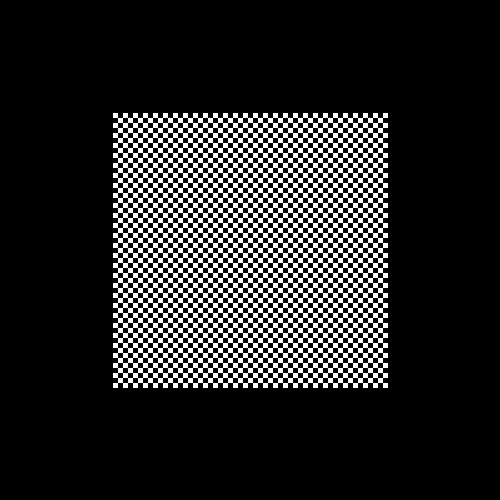
\includegraphics[scale=0.2]{checker_fine_large}
			\caption{Large chessboard}
			\label{subfig:b}
		\end{subfigure}	
		\\
		\begin{subfigure}{0.2\textwidth}
			
\includegraphics[scale=0.2]{square_small}
			\caption{Small square}
			\label{subfig:c}
		\end{subfigure}		
		~
		\begin{subfigure}{0.2\textwidth}
			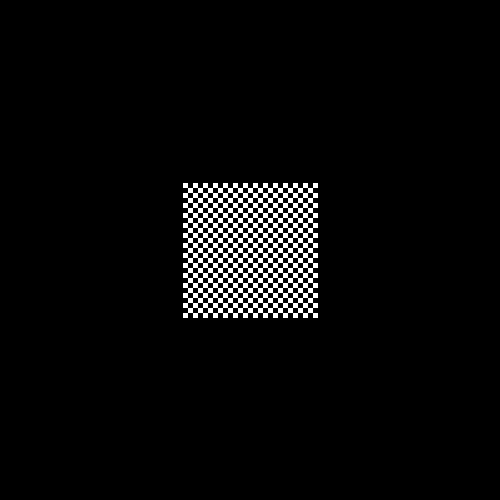
\includegraphics[scale=0.2]{checker_fine_small}
			\caption{Small chessboard}
			\label{subfig:d}
		\end{subfigure}	
	
		\caption{The total white area is identical for both the large and the small shapes respectively. Horizontal comparison alows to evaluate density, vertical comparison alows to evaluate size. }
		\label{fig:v}
		
	\end{center}
\end{figure}

\FloatBarrier

{\parindent0pt   % starts non-indentation

For each of those four images, we imposed four different types of modifications, each performed with small steps, as large deviations between a created segmentation and a given ground truth can already be determined by the naked eye and thus do not require an evaluation metric.

\hspace{1in}

\subsubsection{Planar shift}
The images were shifted by 1 through 5 pixels in steps of 1 pixel. This will be the main basis for comparison, as it turned out to be the most linear and consistent type of modification.
	
\subsubsection{Upscale and downscale}
The images were scaled by 1 through 5 percent in steps of 1 percent. This was done both for upscaling and downscaling. Upscaling changes the segment by adding false positive (FP) values, while downscaling changes the segment by adding false negative (FN) values.

\subsubsection{Blurring the edges}
The edges of the features inside the images were blurred, by exchanging random pixels in a defined distance within the image. This distance was varied by 1 through 5 pixels in steps of 1 pixel. This changes the border of the segment clusters in a different way than the scaling does.

\subsubsection{Rotation}
The images were rotated by 1 through 5 degrees in steps of 1 degree. Works as an approach but the interpolation makes changes inconsistent for small angles.

} % ends non-indentation



\clearpage

\section{Results}
\label{Results}

To present our results in a clear manner, we will classify them by the types of metrics we looked at. The results are presented as they are and the appropriate conclusions are drawn from the measurements, as well as from literature, for each metric respectively. The consequence of these results are later on discussed in more detail in chapter IV: Discussion and their essence are synthesized in chapter V: Conclusion.

\subsection{Overlap based evaluation metrics}

Overlap based evaluation metrics are the most intuitive type of metric to understand. The segmentation and the ground truth are overlayed and each pixel in the segmentation is compared to the corresponding pixel in the ground truth. Depending on the two values the pixel position gets one of four states assigned.

\hspace{1in}

{\parindent0pt   % starts non-indentation
		
\subsubsection{True Positive}
If the segmentation defines the pixel as belonging to the feature and the ground truth says the pixel belongs to the feature, the pixel is classified as True Positive (TP).

\subsubsection{False Positive}
If the segmentation defines the pixel as belonging to the feature and the ground truth says the pixel belongs to the background, the pixel is classified as False Positive (FP).

\subsubsection{True Negative}
If the segmentation defines the pixel as belonging to the background and the ground truth says the pixel belongs to the background, the pixel is classified as True Negative (TN). Metrics considering the true negatives have a strong dependence on the amount of background in the image and with that a sensitivity to the feature size.

\subsubsection{False Negative}
If the segmentation defines the pixel as belonging to the background and the ground truth says the pixel belongs to the feature, the pixel is classified as False Negative (FN).

} % ends non-indentation

\hspace{1in}

After each pixel has been assigned to a cardinality, they are summed up and their results are stored in the so-called confusion matrix.

\begin{center}
	\begin{tabular}{|l| c |r| }
		\hline
		True Positive & False Positive \\ \hline
		False Negative & True Negative \\
		\hline
	\end{tabular}
	\captionof{table}{Confusion Matrix}
\end{center}

The most important overlap based metric, we are going to talk about is the F- Measure. The F-Measure takes the sensitivity (TPR) and the precision (PPV) into consideration, which both are based on the confusion matrix, and weights them according to a factor \(\beta\). The DICE is the special case of the F-Measure for which \( \beta \) is equal to 1. 

\begin{multicols}{2}	% Equation TPR and PPV
	\begin{equation}
		TPR = \frac{TP}{TP+TN} 
	\end{equation} 
	\break
	\begin{equation}
		PPV = \frac{TP}{TP + FP} 
	\end{equation}
\end{multicols}

\begin{equation}	% Equation FMS
	FMS_{\beta} = \frac{(\beta^2+1) \cdot PPV \cdot TPR}{ \beta^2 \cdot PPV + TPR}
\end{equation}

\hspace{2in}

The DICE ist the most commonly used evaluation metric. Depending on the circumstance one could desire a metric such as the Jaccard index (JAC), which is based on the DICE but reacts more sensitive to changes.

\begin{equation} % Equation JAC
JAC = \frac{DICE}{2-DICE}
\end{equation}

To show the relationship between the DICE and the Jaccard index we compare them directly. Below their reaction to the large square is shown.

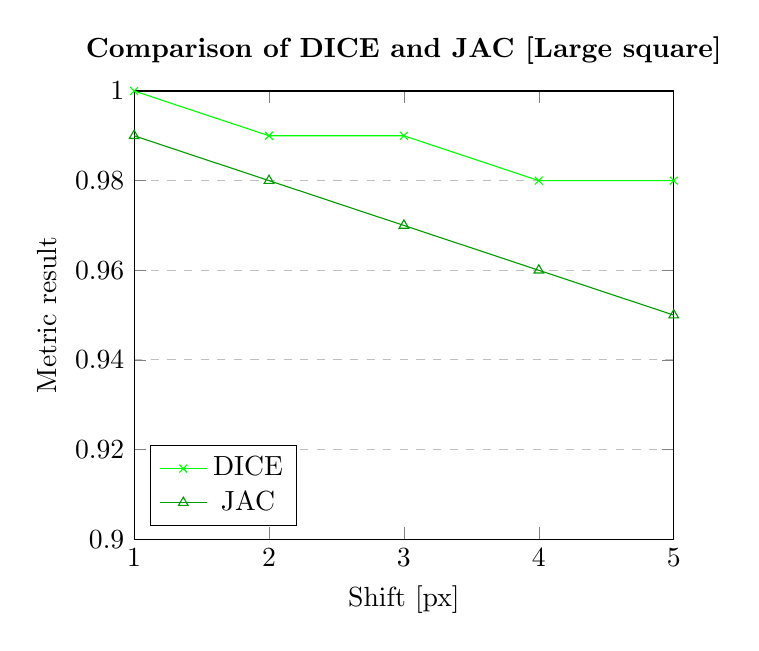
\begin{tikzpicture} % Comparison of DICE and JAC [Large square]
\begin{axis}[
title = {\textbf{Comparison of DICE and JAC [Large square]}},
xlabel = {Shift [px]},
ylabel = {Metric result},
xmin = 1, xmax = 5,
ymin = 0.9, ymax = 1,
xtick = {1,2,3,4,5},
ytick = {},
legend pos = south west,
ymajorgrids = true,
grid style = dashed,		
]

\addplot[color = DICE,mark = x]
coordinates{(1,1.00)(2,0.99)(3,0.99)(4,0.98)(5,0.98)	};

\addplot[color = JAC,mark = triangle]
coordinates{(1,0.99)(2,0.98)(3,0.97)(4,0.96)(5,0.95)	};

\legend{DICE, JAC}

\end{axis}
\end{tikzpicture}

We can see, that the Jaccard index reacts stronger to the same change than the DICE does and this is independent of the type of change, as this behavior could be observed in all our measurements.

\hspace{1in}

For further tests, we limit the representation to the DICE as it is the most used of the two metrics and they depend mathematically on each other. We investigated then further the influence of feature size and density for the DICE, which yielded the following results confirming our expectations:

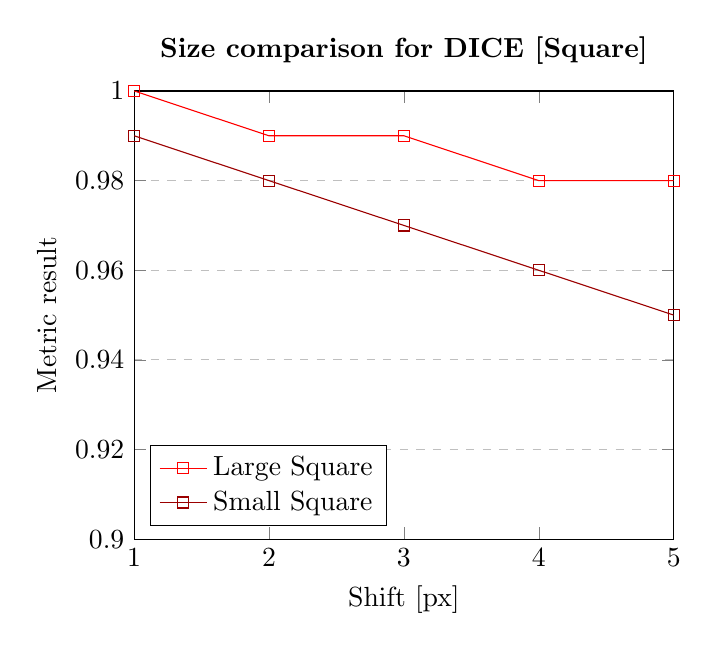
\begin{tikzpicture} % Size comparison for DICE [Square]
	\begin{axis}[
		title = {\textbf{Size comparison for DICE [Square]}},
		xlabel = {Shift [px]},
		ylabel = {Metric result},
		xmin = 1, xmax = 5,
		ymin = 0.9, ymax = 1,
		xtick = {1,2,3,4,5},
		ytick = {},
		legend pos = south west,
		ymajorgrids = true,
		grid style = dashed,		
		]
		
		\addplot[color = Square_Large,mark = square]
		coordinates{(1,1.00)(2,0.99)(3,0.99)(4,0.98)(5,0.98)	};
	
		\addplot[color = Square_Small,mark = square]
		coordinates{(1,0.99)(2,0.98)(3,0.97)(4,0.96)(5,0.95)	};
	
		\legend{Large Square, Small Square}
		
	\end{axis}
\end{tikzpicture}

Similiar to how the Jaccard index reacts more sensitive than the DICE on an identical image, the DICE reacts more sensitive on smaller features, as this size comparison shows.

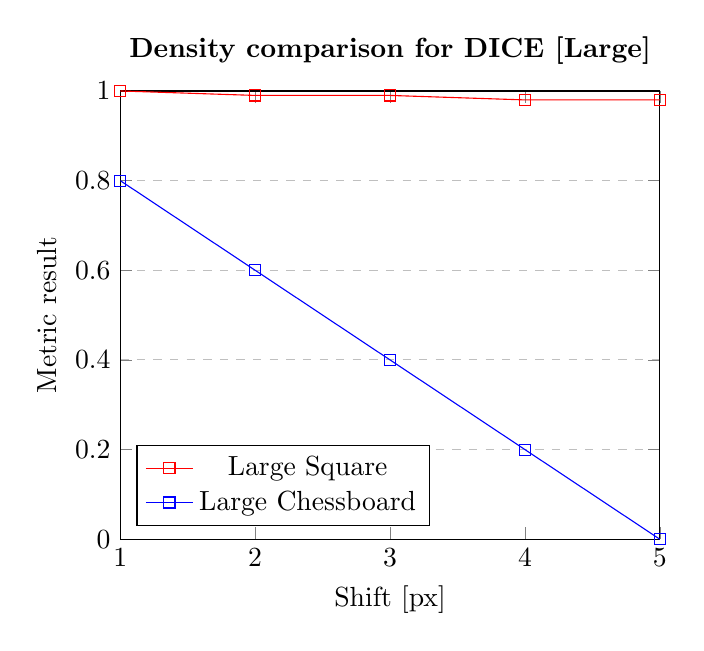
\begin{tikzpicture} % Density comparison for DICE [Large]
\begin{axis}[
title = {\textbf{Density comparison for DICE [Large]}},
xlabel = {Shift [px]},
ylabel = {Metric result},
xmin = 1, xmax = 5,
ymin = 0, ymax = 1,
xtick = {1,2,3,4,5},
ytick = {},
legend pos = south west,
ymajorgrids = true,
grid style = dashed,		
]

\addplot[color = Square_Large,mark = square]
coordinates{(1,1.00)(2,0.99)(3,0.99)(4,0.98)(5,0.98)	};

\addplot[color = Chess_Large,mark = square]
coordinates{(1,0.80)(2,0.60)(3,0.40)(4,0.20)(5,0.00)	};

\legend{Large Square, Large Chessboard}

\end{axis}
\end{tikzpicture}

This measurement clearly shows the extreme dependance of the DICE on high feature density, as a small change between the segmentation and the ground truth, already changes the result of the DICE drastically.

\subsection{Probabilistic evaluation metrics}

In contrast to the overlap based evaluation metrics, the ones based on a probability measure the correlation between the two segments, rather than just evaluating how good the areas overlap. Correlation is a statistical relationship, that determines to how close the relationship between two segments to a linear relation is.

\hspace{2in}

The first probabilistic evaluation metric we looked at was the Interclass Correlation (ICC) given by the following formula, with \(\sigma_S \) as the variance caused by the differences between the segmentation and the ground truth and \(\sigma_\epsilon \) as the variance caused by differences between the points of the segmentation and the ground truth.

\begin{equation} % Equation of ICC
	ICC = \frac{\sigma_S^2}{\sigma_S^2 + \sigma_\epsilon^2}
\end{equation}

The second probabilistic evaluation metric we investigated was the Probabilistic Distance (PBD) given by the formula below, with $P_S$ and $P_G$ are the probability distributions of the segmentation and the ground truth respectively and $P_SG$ being their joint probability distribution.

\begin{equation} % Equation of PBD
	PBD(S,G) = \frac{\int |P_S - P_G| }{2 \int P_{SG}}
\end{equation}

Both of these metrics displayed the same sensibility as the overlap based metrics to the size and even stronger sensibility to the density. This is shown in the two figures below, as the interclass correlation and the probabilistic distance are plotted against the DICE for comparison.

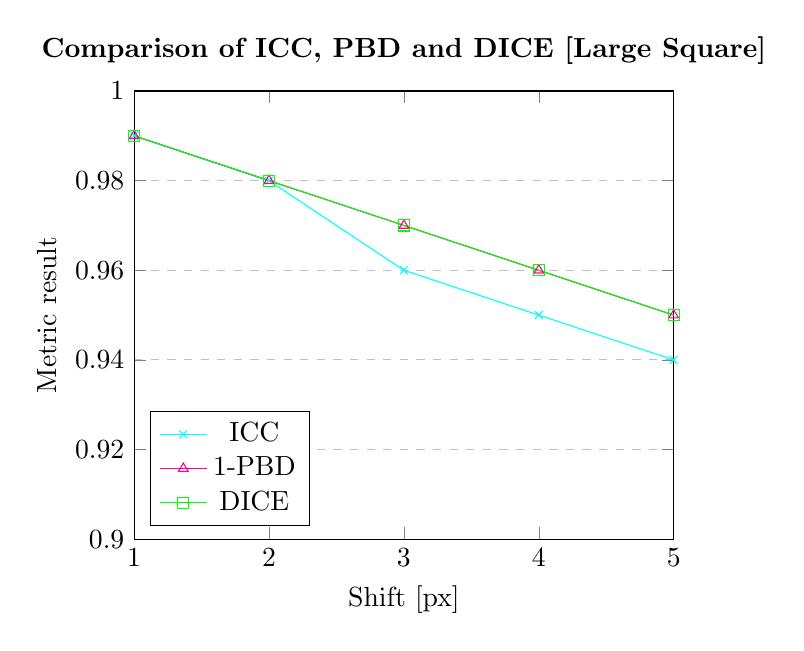
\begin{tikzpicture} % Comparison of ICC, PBD and DICE [Large Square]
\begin{axis}[
title = {\textbf{Comparison of ICC, PBD and DICE [Large Square]}},
xlabel = {Shift [px]},
ylabel = {Metric result},
xmin = 1, xmax = 5,
ymin = 0.9, ymax = 1,
xtick = {1,2,3,4,5},
ytick = {0.9,0.92, 0.94, 0.96, 0.98,1},
legend pos = south west,
ymajorgrids = true,
grid style = dashed,		
]

\addplot[color = ICC,mark = x]
coordinates{(1,0.99)(2,0.98)(3,0.96)(4,0.95)(5,0.94)	};

\addplot[color = PBD,mark = triangle]
coordinates{(1,0.99)(2,0.98)(3,0.97)(4,0.96)(5,0.95)	};

\addplot[color = DICE,mark = square]
coordinates{(1,0.99)(2,0.98)(3,0.97)(4,0.96)(5,0.95)	};

\legend{ICC, 1-PBD, DICE}

\end{axis}
\end{tikzpicture}

This figure shows the reaction of the three metrics to the small square, the reaction to the big square is analogous to the small one, except smaller (See Size comparison for DICE). From the measurements, we were able to deduct, that both the interclass correlation and the probabilistic distance react about equal to the DICE, which makes them redundant metric choices in this perspective.

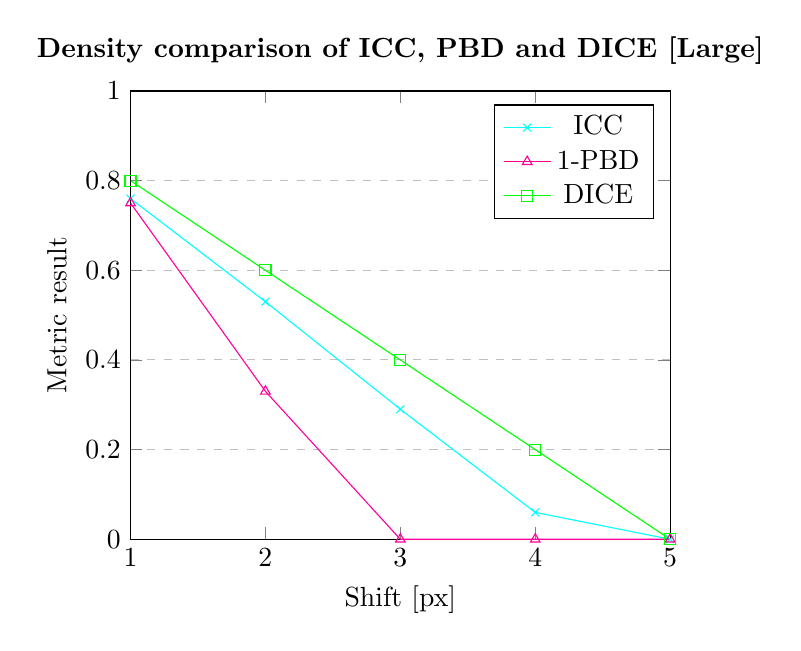
\begin{tikzpicture} % Density comparison of ICC, PBD and DICE [Large]
\begin{axis}[
title = {\textbf{Density comparison of ICC, PBD and DICE [Large]}},
xlabel = {Shift [px]},
ylabel = {Metric result},
xmin = 1, xmax = 5,
ymin = 0, ymax = 1,
xtick = {1,2,3,4,5},
ytick = {},
legend pos = north east,
ymajorgrids = true,
grid style = dashed,		
]

\addplot[color = ICC,mark = x]
coordinates{(1,0.76)(2,0.53)(3,0.29)(4,0.06)(5,0.00)	};

\addplot[color = PBD,mark = triangle]
coordinates{(1,0.75)(2,0.33)(3,0.00)(4,0.00)(5,0.00)	};

\addplot[color = DICE,mark = square]
coordinates{(1,0.80)(2,0.60)(3,0.40)(4,0.20)(5,0.00)	};

\legend{ICC, 1-PBD, DICE}

\end{axis}
\end{tikzpicture}

As it can be derived from this figure, the probabilistic metrics react even stronger to changes in the large chessboard than the dice, which makes them even more sensitive to low densities.

\hspace{2in}

The Cohen Kappa Coefficient(KAP) measures how good the agreement between two given segments is. A big advantage of this metric compared to the others is, that it takes changes caused by chance into consideration, however, at the same time, it still suffers from the high sensitivity to size and density, even though a bit less than the others. It considers the agreement between the segmentation and the ground truth $P_a$ and the hypothetical probability, that the two agree by chance $P_c$, as given in the formula below.

\begin{equation} % Equation of KAP
	KAP = \frac{P_a - P_c}{1 - P_c}
\end{equation}

The Area Under Curve (AUC) considers the fallout (FPR) and the complementarily (FNR), which causes it to suffer from the same problems as the other metrics mentioned up until now. 

\begin{equation} % Equation of AUC
	AUC = 1 - \frac{FPR + FNR}{2}
\end{equation}

The Cohen Kappa coefficient and the area under the curve are compared to the other probabilistic metrics less sensitive to density as the following figure will show. Even though the sensitivity falls short of the DICE it is still rather high. In our measurements, it further turned out that the reaction to size was only minimal jet still detectable.

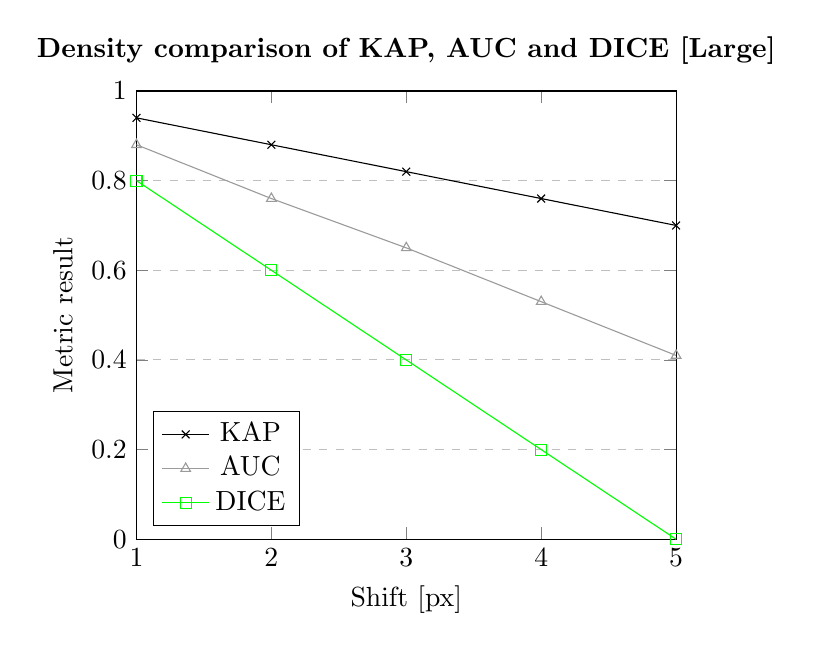
\begin{tikzpicture} % Density comparison of KAP, AUC and DICE [Large]
\begin{axis}[
title = {\textbf{Density comparison of KAP, AUC and DICE [Large]}},
xlabel = {Shift [px]},
ylabel = {Metric result},
xmin = 1, xmax = 5,
ymin = 0, ymax = 1,
xtick = {1,2,3,4,5},
ytick = {},
legend pos = south west,
ymajorgrids = true,
grid style = dashed,		
]

\addplot[color = KAP,mark = x]
coordinates{(1,0.94)(2,0.88)(3,0.82)(4,0.76)(5,0.70)	};

\addplot[color = AUC,mark = triangle]
coordinates{(1,0.88)(2,0.76)(3,0.65)(4,0.53)(5,0.41)	};

\addplot[color = DICE,mark = square]
coordinates{(1,0.80)(2,0.60)(3,0.40)(4,0.20)(5,0.00)	};

\legend{KAP, AUC, DICE}

\end{axis}
\end{tikzpicture}






\subsection{Information theoretic based evaluation metrics}

The Mutual Information (MI) measures the amount of information the segmentation contains about the ground truth and vise versa, or with other words, how similar the two segments are. The formula below is simplified as H(S) corresponds to the entropy of S. The big advantage of this is, that the calculation is region based and not pixel based.

\begin{equation} % Equation of MI
MI = H(S_g) + H(S_t) - H(S_g,S_t)
\end{equation}

\begin{equation} % Equation of VOI
VOI =2 H(S_g) + 2H(S_t) - 3H(S_g,S_t)
\end{equation}

The Variation of Information (VOI) is a modification of the MI, as it effectively measures the change of information between the segments (loss or gain). Since the variation of information is derived from the mutual information, we will primarily consider the mutual information in our representation going forward.

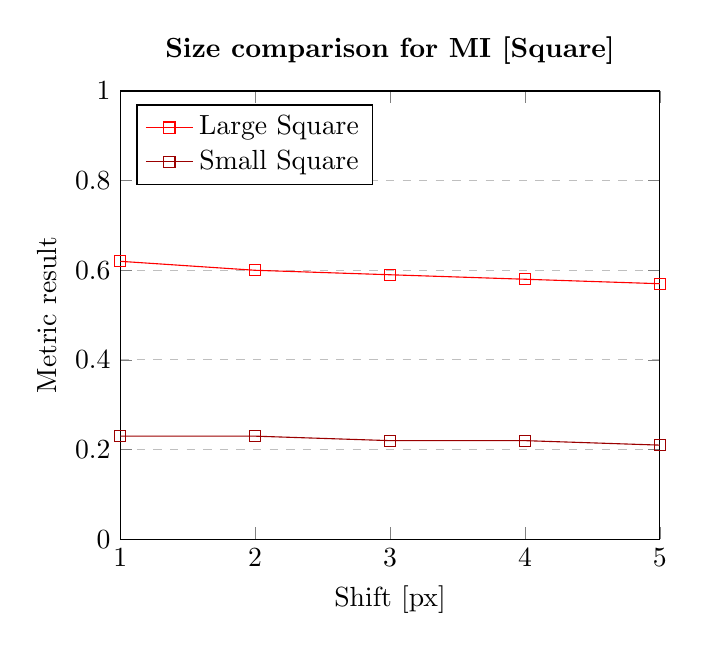
\begin{tikzpicture} % Size comparison for MI [Square]
\begin{axis}[
title = {\textbf{Size comparison for MI [Square]}},
xlabel = {Shift [px]},
ylabel = {Metric result},
xmin = 1, xmax = 5,
ymin = 0, ymax = 1,
xtick = {1,2,3,4,5},
ytick = {},
legend pos = north west,
ymajorgrids = true,
grid style = dashed,		
]

\addplot[color = Square_Large,mark = square]
coordinates{(1,0.62)(2,0.60)(3,0.59)(4,0.58)(5,0.57)	};

\addplot[color = Square_Small,mark = square]
coordinates{(1,0.23)(2,0.23)(3,0.22)(4,0.22)(5,0.21)	};

\legend{Large Square, Small Square}

\end{axis}
\end{tikzpicture}

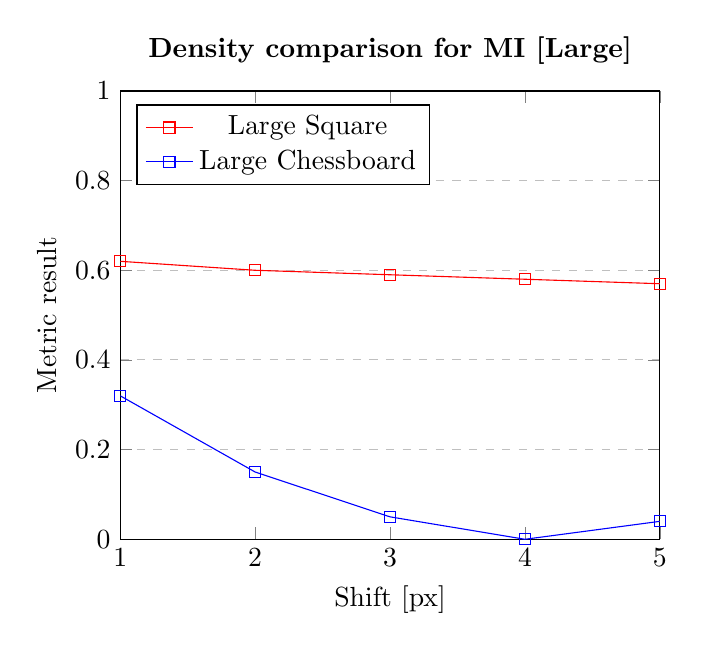
\begin{tikzpicture} % Density comparison for MI [Large]
\begin{axis}[
title = {\textbf{Density comparison for MI [Large]}},
xlabel = {Shift [px]},
ylabel = {Metric result},
xmin = 1, xmax = 5,
ymin = 0, ymax = 1,
xtick = {1,2,3,4,5},
ytick = {},
legend pos = north west,
ymajorgrids = true,
grid style = dashed,		
]

\addplot[color = Square_Large,mark = square]
coordinates{(1,0.62)(2,0.60)(3,0.59)(4,0.58)(5,0.57)	};

\addplot[color = Chess_Large,mark = square]
coordinates{(1,0.32)(2,0.15)(3,0.05)(4,0.00)(5,0.04)	};

\legend{Large Square,Large Chessboard}

\end{axis}
\end{tikzpicture}

Our measurements have shown, that both these metrics react strongly to changes in size and density, however, they react only slightly to modifications of the image. This can be seen in the two figures above.






\subsection{Pair counting based evaluation metrics}

The Rand Index (RI) measures the similarity between two clusters, one taken from the segmentation and one from the ground truth. The comparison is mathematically related to the accuracy, but the important difference is, that the Rand index is not label based, so it can even be used when no labels are in place. In the equation given below (a+b) can be considered the total number of agreements and (c+d) can be considered the total number of disagreements between the segmentation and the ground truth.

\begin{equation} % Equation of RI
	RI = \frac{a+b}{a+b+c+d}
\end{equation}

The modification of the RI is the Adjusted Rand Index (ARI), which corrects the RI for influences caused by chance.

\begin{equation} % Equation of ARI
	ARI = \frac{2(ad-bc)}{c^2 + b^2 + 2ad + (a+d)(c+b)}
\end{equation}

The Rand index showed only a small reaction to changes in size and density, the adjusted Rand index, on the other hand, showed stronger reactions.

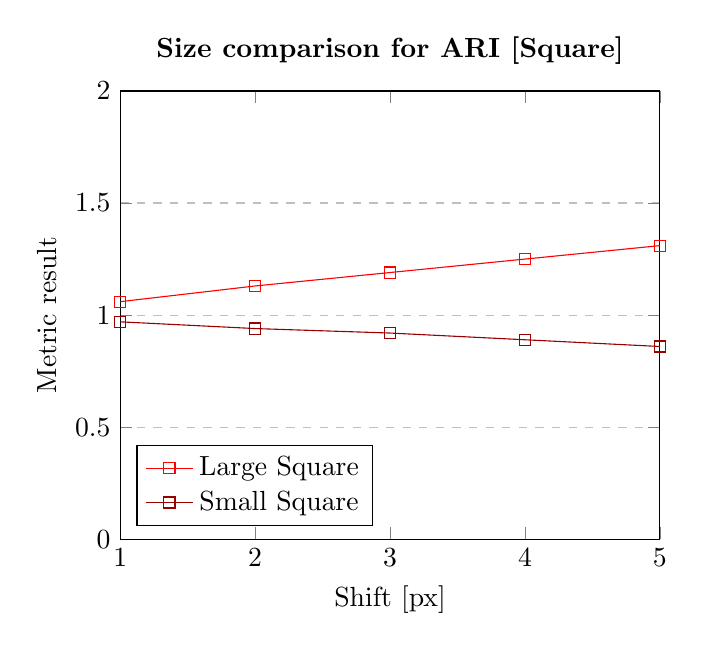
\begin{tikzpicture} % Size comparison for ARI [Square]
\begin{axis}[
title = {\textbf{Size comparison for ARI [Square]}},
xlabel = {Shift [px]},
ylabel = {Metric result},
xmin = 1, xmax = 5,
ymin = 0, ymax = 2,
xtick = {1,2,3,4,5},
ytick = {},
legend pos = south west,
ymajorgrids = true,
grid style = dashed,		
]

\addplot[color = Square_Large,mark = square]
coordinates{(1,1.06)(2,1.13)(3,1.19)(4,1.25)(5,1.31)	};

\addplot[color = Square_Small,mark = square]
coordinates{(1,0.97)(2,0.94)(3,0.92)(4,0.89)(5,0.86)	};

\legend{Large Square, Small Square}

\end{axis}
\end{tikzpicture}

This figure shows a dependance size, as it was the case for all metrics until this point.

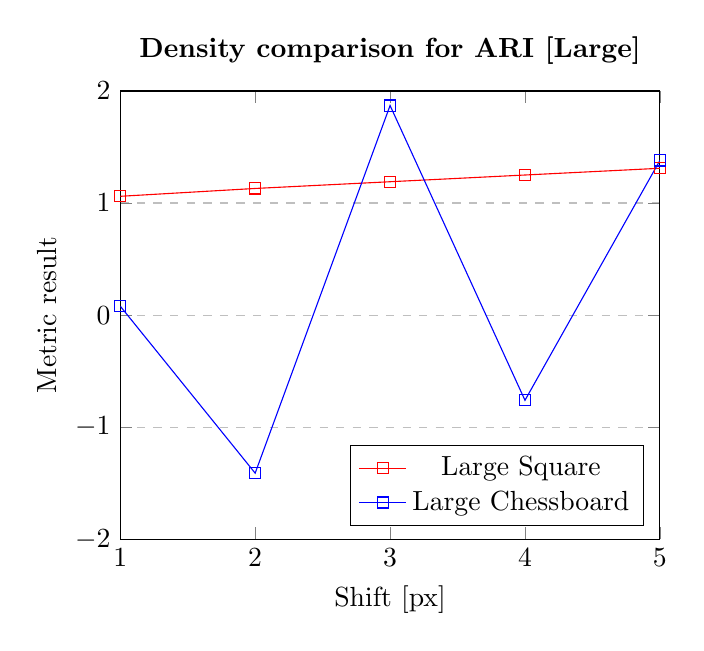
\begin{tikzpicture} % Density comparison for ARI [Large]
\begin{axis}[
title = {\textbf{Density comparison for ARI [Large]}},
xlabel = {Shift [px]},
ylabel = {Metric result},
xmin = 1, xmax = 5,
ymin = -2, ymax = 2,
xtick = {1,2,3,4,5},
ytick = {},
legend pos = south east,
ymajorgrids = true,
grid style = dashed,		
]

\addplot[color = Square_Large,mark = square]
coordinates{(1,1.06)(2,1.13)(3,1.19)(4,1.25)(5,1.31)	};

\addplot[color = Chess_Large,mark = square]
coordinates{(1,0.08)(2,-1.41)(3,1.87)(4,-0.76)(5,1.38)	};

\legend{Large Square,Large Chessboard}

\end{axis}
\end{tikzpicture}

In this figure a very strong dependence on the density can be seen, as the small changes within the chessboard image cause extreme variation in the adjusted Rand index.





\subsection{Spacial distance based evaluation metrics}

The Hausdorff Distance (HD) measures the distance between two given subsets. The distance then is defined as the difference between the two closest points and the two points the most far away between the two subsets. This has the effect, that outliers are strongly taken into consideration, an effect, that no metric until now has displayed. Depending on the application, this can be sought after, for example, to empathize on the boundaries, but mostly this is a hindrance. Our measurements clearly showed this behavior, as changes to the boundary had a tremendous effect, while other changes did almost nothing.

The Average Hausdorff Distance (AVD), calculates all distances in the subsets and averages over them, to account for the outliers. This makes it more stable and an overall better choice than the regular Hausdorff distance, if the outlier sensitivity is not desired.

\hspace{2in}

Slight changes, such as rotation or shifting the image, as it was the most effective modification throughout all other metrics, showed almost no reaction, as the Hausdorff distance detected no big change. Where reaction could be observed was if changes happened primarily to the boundary of the image, such as blurring the edges and scaling the image.

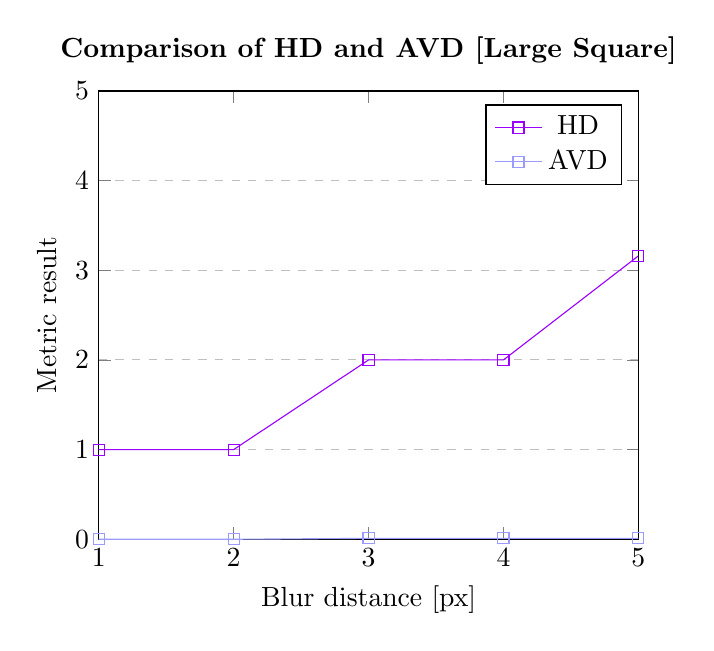
\begin{tikzpicture} % Comparison of HD and AVD [Large Square]
\begin{axis}[
title = {\textbf{Comparison of HD and AVD [Large Square]}},
xlabel = {Blur distance [px]},
ylabel = {Metric result},
xmin = 1, xmax = 5,
ymin = 0, ymax = 5,
xtick = {1,2,3,4,5},
ytick = {},
legend pos = north east,
ymajorgrids = true,
grid style = dashed,		
]

\addplot[color = HD,mark = square]
coordinates{(1,1.00)(2,1.00)(3,2.00)(4,2.00)(5,3.16)	};

\addplot[color = AVD,mark = square]
coordinates{(1,0.00)(2,0.00)(3,0.01)(4,0.01)(5,0.01)	};

\legend{HD, AVD}

\end{axis}
\end{tikzpicture}

By blurring the edges slightly the Hausdorff distance reacts, whereas the averaged Hausdorff distance detects only a minimal modification. The blur as modification adds to the same extend new FP and FN and this happens equally around the square so that these changes overall seem to negate each other. If they would not, something like in the figure below can be observed.

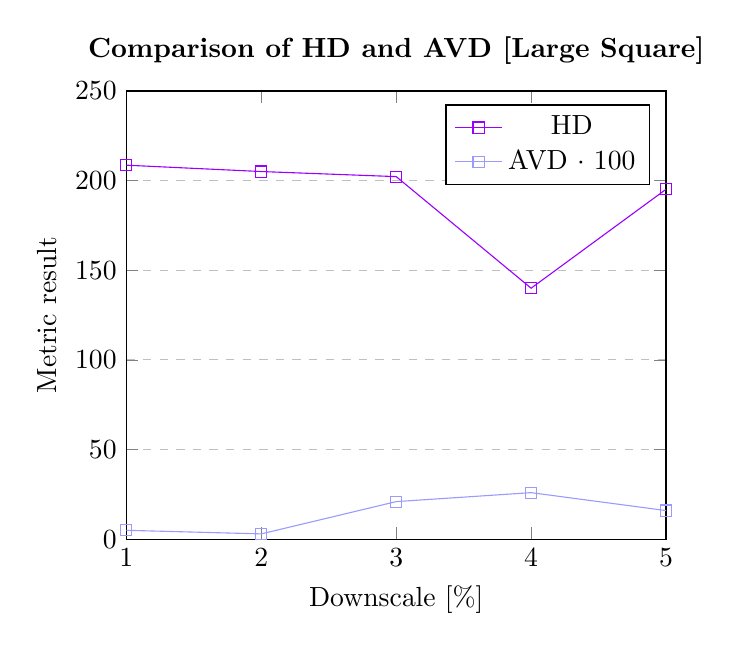
\begin{tikzpicture} % Comparison of HD and AVD [Large Square]
\begin{axis}[
title = {\textbf{Comparison of HD and AVD [Large Square]}},
xlabel = {Downscale [\%]},
ylabel = {Metric result},
xmin = 1, xmax = 5,
ymin = 0, ymax = 250,
xtick = {1,2,3,4,5},
ytick = {},
legend pos = north east,
ymajorgrids = true,
grid style = dashed,		
]

\addplot[color = HD,mark = square]
coordinates{(1,208.6)(2,205.06)(3,202.23)(4,140.00)(5,195.16)	};

\addplot[color = AVD,mark = square]
coordinates{(1,5)(2,3)(3,21)(4,26)(5,16)	};

\legend{HD, AVD \(\cdot\) 100}

\end{axis}
\end{tikzpicture}

Special emphasis is to be given to the scale of this figure compared to the figure above this one. The downscale modification adds one layer of FN all around the square, which adds up to an extremely high value for the Hausdorff distance. Here becomes the difference between the Hausdorff distance and the averaged Hausdorff distance evident, as the later had to be scaled a hundredfold just to be visible in the plot.

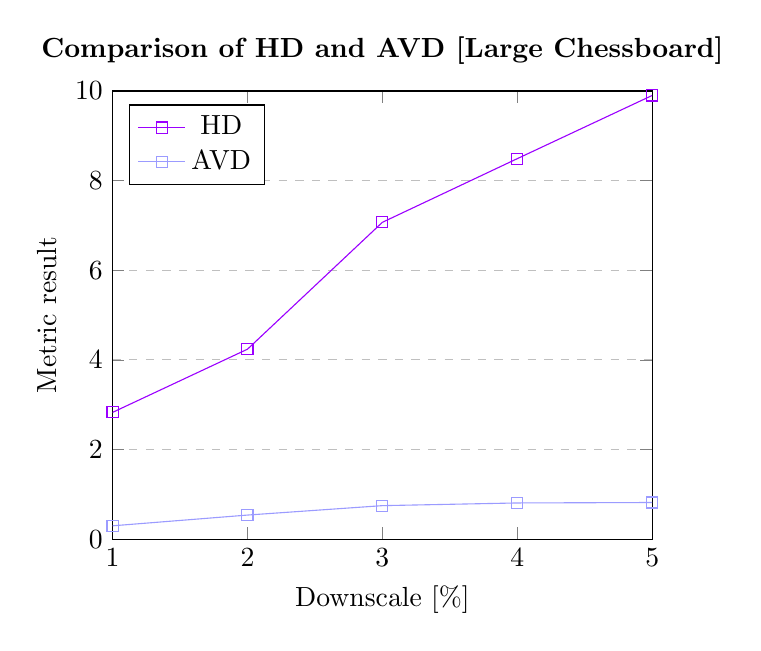
\begin{tikzpicture} % Comparison of HD and AVD [Large Chessboard]
\begin{axis}[
title = {\textbf{Comparison of HD and AVD [Large Chessboard]}},
xlabel = {Downscale [\%]},
ylabel = {Metric result},
xmin = 1, xmax = 5,
ymin = 0, ymax = 10,
xtick = {1,2,3,4,5},
ytick = {},
legend pos = north west,
ymajorgrids = true,
grid style = dashed,		
]

\addplot[color = HD,mark = square]
coordinates{(1,2.83)(2,4.24)(3,7.07)(4,8.49)(5,9.90)	};

\addplot[color = AVD,mark = square]
coordinates{(1,0.30)(2,0.54)(3,0.75)(4,0.81)(5,0.82)	};

\legend{HD, AVD}


\end{axis}
\end{tikzpicture}

Apart from the dependence of the boundary of the Hausdorff distance, both metrics seem to be uninfluenced by size or density, as this figure shows quite a similar behavior to the square.

\hspace{2in}

The other spacial distance based metric we looked at, was the Mahalanobis Distance (MHD). While it works similar to the Hausdorff distance it also considers the spacial position of the false negatives (FN) and the false positives (FP), not just the spacial position the true positives (TP) and/or the true negatives (TN) like most other spacial metrics do. In essence, this makes the Mahalanobis Distance one of the best-structured evaluation metrics. 

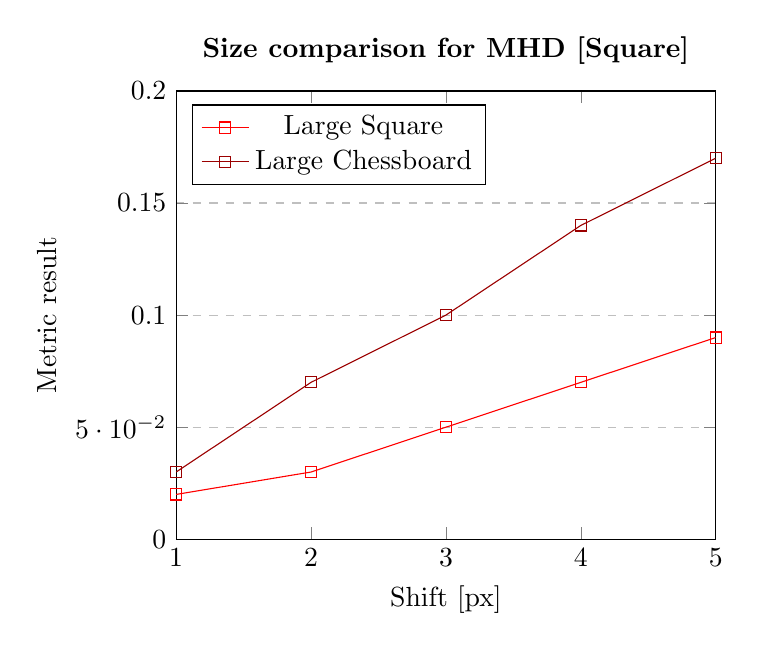
\begin{tikzpicture} % Size comparison for MHD [Square]
\begin{axis}[
title = {\textbf{Size comparison for MHD [Square]}},
xlabel = {Shift [px]},
ylabel = {Metric result},
xmin = 1, xmax = 5,
ymin = 0, ymax = 0.2,
xtick = {1,2,3,4,5},
ytick = {},
legend pos = north west,
ymajorgrids = true,
grid style = dashed,		
]

\addplot[color = Square_Large,mark = square]
coordinates{(1,0.02)(2,0.03)(3,0.05)(4,0.07)(5,0.09)	};

\addplot[color = Square_Small,mark = square]
coordinates{(1,0.03)(2,0.07)(3,0.10)(4,0.14)(5,0.17)	};

\legend{Large Square,Large Chessboard}

\end{axis}
\end{tikzpicture}

The influence of the size is quite small compared to what other metrics have shown.

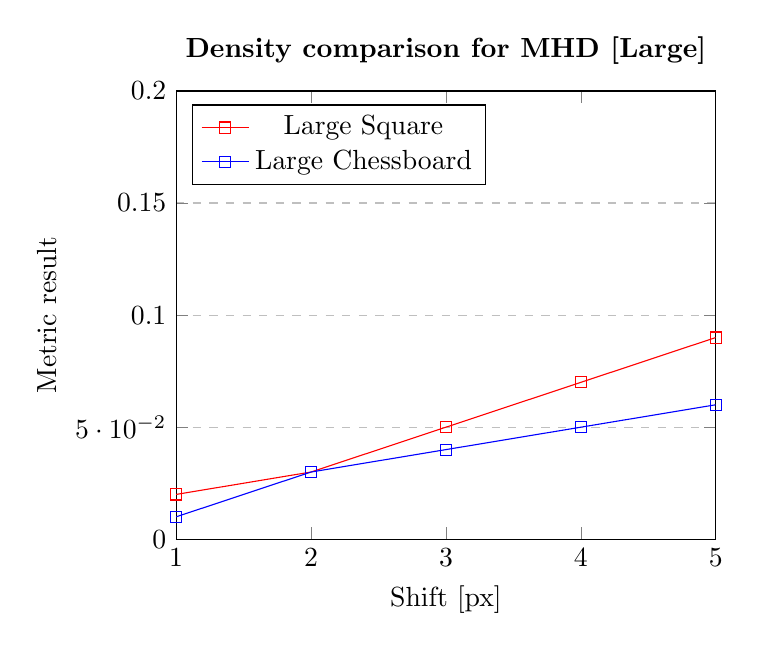
\begin{tikzpicture} % Density comparison for MHD [Large]
\begin{axis}[
title = {\textbf{Density comparison for MHD [Large]}},
xlabel = {Shift [px]},
ylabel = {Metric result},
xmin = 1, xmax = 5,
ymin = 0, ymax = 0.2,
xtick = {1,2,3,4,5},
ytick = {},
legend pos = north west,
ymajorgrids = true,
grid style = dashed,		
]

\addplot[color = Square_Large,mark = square]
coordinates{(1,0.02)(2,0.03)(3,0.05)(4,0.07)(5,0.09)	};

\addplot[color = Chess_Large,mark = square]
coordinates{(1,0.01)(2,0.03)(3,0.04)(4,0.05)(5,0.06)	};

\legend{Large Square,Large Chessboard}

\end{axis}
\end{tikzpicture}
 
In this figure, it becomes evident that the Mahalanobis distance is not at all influenced by the density of the feature.
 
 
 

\subsection{Volume based evaluation metrics}
Since all our tests were performed on two-dimensional images, we could not deliver results for the volume based evaluation metrics, however, it is the metric of choice, if the general alignment of the whole volume is the most important requirement, as every other metric does not provide such a functionality.


\clearpage

\section{Discussion}
\label{Discussion}

Our measurements have shown, that almost all metrics have a medium to a strong dependency on the size and density of the feature present in the image. However this does not automatically exclude these metrics from being used, one just has to be aware of their weaknesses.

\hspace{2in}

{\parindent0pt   % starts non-indentation

\subsubsection{Overlap based evaluation metrics}
If the general alignment of the segmentation and the ground truth can be guaranteed, then the overlap based metrics can be utilized to detect even the smallest deviations between the segmentation and the ground truth. This makes them perfect evaluation metrics to polish the last bit of the algorithm used to match the segmentation on the ground truth. This means, however, that these metrics highly depend on the existence of a ground truth for testing. Furthermore, these metrics are all stable against outliers and boundary effects.

\subsubsection{Probabilistic evaluation metrics}
These metrics are about equal in dependency on the feature size, as the overlap based metrics are, but they react quite differently to the density. As one part of the probabilistic metrics reacts more, the other part reacts less than the overlap based metrics (here Cohens Kappa coefficient excels over the others as it considers chance in its computations). In the end the results of these metrics are comparable to the overlap based metrics, however, they need much more computational effort, which might have to be considered, if whole body volumes would be evaluated. These metrics as well are stable against outliers and boundary effects. They also work best if the general alignment is given and on the premise that a ground truth is given.

\subsubsection{Information theoretic based evaluation metrics}
The entropy as a means to measure correlation works fine, but is also quite calculation intensive, especially compared to the computational effort of the overlap based metrics. The reaction to size and density are as it is for the overlap and probabilistic metrics as well. The main advantage of these metrics over the others is that they can be used to compare consecutive segmentations to determine changes in between segmentations. This is especially useful if no real ground truth exists.

\subsubsection{Pair counting based evaluation metrics}
While the adjusted Rand index also takes the chance into consideration, the sensitivity to size and especially the sensitivity to density are quite bad. One might consider using these metrics, as they require less computational effort than the information theoretic based and the probabilistic metrics, while still considering more relations than the overlay based metrics. This is possible since these metrics only considers clusters and not the whole segmentation.

\subsubsection{Spacial distance based evaluation metrics}
These metrics deliver by far the best overall results and can be used in almost every case mentioned above, without a problem. The only exception being the Hausdorff distance, which reacts sensitively to outliers. The averaged Hausdorff distance is capable of identifying every type of modification we imposed, while still being independent of size and density, which makes it a great all-around metric. The only problem with the averaged Hausdorff distance is, that it can not guarantee good alignment of the segmentation and the ground truth. The Mahalanobis distance is the only tested metric, capable of securely determine correct alignment of the segmentation and the ground truth. This ability is independent of size and density of the features. However, the Mahalanobis distance has difficulties if the boundaries become too complex.

} % ends non-indentation






\section{Conclusion}
\label{Conclusion}

Based on our measurements, which support the findings of other literature such as the paper published by A.Taha and A.Hanbury, with the goal to segment brain scans, we recommend to use a combination of the Mahalanobis distance, averaged Hausdorff distance and the DICE.

\hspace{2in}

The Mahalanobis distance is the only metric that guarantees correct alignment of the segmentation and the ground truth, while the averaged Hausdorff distance, determines the detailed alignment. The averaged Hausdorff distance is superior to the DICE, as the DICE is strongly influenced by feature size and density. The reason why the DICE is still used is that under the right conditions it is absolutely viable and also it is probably the most referenced metric in publications, so it offers a value to compare to the literature.



% if have a single appendix:
%\appendix[Proof of the Zonklar Equations]
% or
%\appendix  % for no appendix heading
% do not use \section anymore after \appendix, only \section*
% is possibly needed

% use appendices with more than one appendix
% then use \section to start each appendix
% you must declare a \section before using any
% \subsection or using \label (\appendices by itself
% starts a section numbered zero.)
%


\appendices
\section{as png}
Database: Images with modifications

\section{as excel/ods}
Measurements and corresponding data evaluation

% Can use something like this to put references on a page
% by themselves when using endfloat and the captionsoff option.
\ifCLASSOPTIONcaptionsoff
  \newpage
\fi



% trigger a \newpage just before the given reference
% number - used to balance the columns on the last page
% adjust value as needed - may need to be readjusted if
% the document is modified later
%\IEEEtriggeratref{8}
% The "triggered" command can be changed if desired:
%\IEEEtriggercmd{\enlargethispage{-5in}}

% references section

% can use a bibliography generated by BibTeX as a .bbl file
% BibTeX documentation can be easily obtained at:
% http://mirror.ctan.org/biblio/bibtex/contrib/doc/
% The IEEEtran BibTeX style support page is at:
% http://www.michaelshell.org/tex/ieeetran/bibtex/
%\bibliographystyle{IEEEtran}
% argument is your BibTeX string definitions and bibliography database(s)
%\bibliography{IEEEabrv,../bib/paper}
%
% <OR> manually copy in the resultant .bbl file
% set second argument of \begin to the number of references
% (used to reserve space for the reference number labels box)
\begin{thebibliography}{1}

\bibitem{IEEEhowto:kopka}

A.~Taha and A.~Hanbury, \emph{Metrics for evaluating 3D medical image segmentation:analysis, selection and tool}.\hskip 1em plus
0.5em minus 0.4em\relax Vienna, Austria: BioMed Central, 2015.




\end{thebibliography}

% biography section
% 
% If you have an EPS/PDF photo (graphicx package needed) extra braces are
% needed around the contents of the optional argument to biography to prevent
% the LaTeX parser from getting confused when it sees the complicated
% \includegraphics command within an optional argument. (You could create
% your own custom macro containing the \includegraphics command to make things
% simpler here.)

% that's all folks
\end{document}


